\documentclass[11pt,american,czech]{article}
\usepackage[T1]{fontenc}
\usepackage[utf8]{inputenc}
\usepackage[a4paper]{geometry}
\geometry{verbose,tmargin=4cm,bmargin=3cm,lmargin=3cm,rmargin=2cm,headheight=0.8cm,headsep=1cm,footskip=0.5cm}
\pagestyle{headings}
\setcounter{secnumdepth}{3}
\usepackage{url}
\usepackage{amsmath}
\usepackage{tcolorbox}
\usepackage{bm}
\usepackage{amsthm}
\usepackage{amssymb}
\usepackage{graphicx}
\usepackage{setspace}
\usepackage{mathrsfs}
\usepackage{hyperref}
\usepackage{subcaption}


%commands
\newcommand{\e}{\mathtt{e}} %e
\newcommand{\dx}{\mathtt{d}} %d
\newcommand{\R}{\mathbb{R}} % množina reálných čísel
\newcommand{\N}{\mathbb{N}} % množina přirozených čísel
\newcommand{\E}{\mathbb{E}} % střední hodnota
\newcommand{\VAR}{\mathtt{VAR}} % rozptyl
\newcommand{\Mod}{\mathtt{Mod}} % rozptyl
\newcommand{\amb}{\mathtt{amb}}
\newcommand{\T}{\mathtt{T}} %T rounds played
\newcommand{\supp}{\mathrm{supp}} %supremum

\usepackage{indentfirst}

\begin{document}
	\title{Multi-armed bandit problem}
	\author{Anežka Lhotáková}
	\date{\today}
	\maketitle
	\begin{abstract}
		In probability theory and machine learning, multi-armed bandit problem refers to a model which can be seen as a set of real distributions $\{F_1,\dots,F_K\}$, each distribution being associated with the rewards delivered by one of the $K\in\N^+$ levers. Let $\mu_1,\dots,\mu_K$ be the mean values associated with these reward distributions. The gambler iteratively plays one lever per round and observes the associated reward. The objective is to maximize the sum of the collected rewards. Several strategies or algorithms have been proposed as a solution to this problem in the last two decades. In this project, we will focus on the most popular strategies and their parameter optimization through heuristic approach.
	\end{abstract}
	\section*{Introduction}
	In this paper, model with i.i.d. (independent and identically distributed) rewards is presented. We define
	\begin{itemize}
		\item horizon $\mathtt{H}$ as the number of rounds to be played,
		\item maximum mean reward as $\mu^* = \mathtt{max}\{\mu_1,\mu_2,\dots,\mu_K\},$
		\item regret $\rho$ after $\T$ rounds played as
		$$\rho(\T) = \T\mu^* - \sum_{t=1}^{\T}r_t,$$
		where $r_t$ is the reward in round $t$ ($\rho$ is also a random variable),
		\item expected regret as $\mathbb{E}[\rho(\T)]$,
		\item symbol $\ell_t^i, (i=1,\dots,K$ and $ t=1,\dots,\mathtt{H})$ for the levers.
	\end{itemize}
	The protocol to the model is following:
	\begin{tcolorbox}[colframe=white]
		Given $\mathtt{H}$ rounds to play, considering $K$ levers, in each round $t=1,\dots,\mathtt{H}$:
		\begin{enumerate}
			\item Based on the strategy, the algorithm picks a lever $\ell_t^i$, $i=1,\dots,K$.
			\item Algorithm observes reward $r_t$ for the chosen lever.
			\item If $t<\mathtt{H}$, the algorithm will play again (point 1., $t\to t+1$), otherwise the game is over.
		\end{enumerate}
	\end{tcolorbox}
	The goal is to maximize the total reward over the $\mathtt{H}$ rounds. Above that, we make two important assumptions:
	\begin{itemize}
		\item The algorithm observes only the reward for the selected action, and nothing else.
		\item The reward for each action is  i.i.d. For each lever $\ell^i$, there is a distribution $F_{i}$ over reals, called the reward distribution. Every time the lever is chosen, the reward is sampled independently from its distribution. The reward distributions are initially unknown to the algorithm.
	\end{itemize}
	For better understanding of the model, let us begin with an example. Imagine player walking into a casino with two slot-machines. Both slot-machines $\ell_1,\ell_2$ have their already given distributions $F_1, F_2$. Let the reward $r$ of each slot-machine be given as $r_1\sim F_1=\mathcal{N}(10,3)$ and $r_2\sim F_2=\mathcal{N}(8,4)$. Unfortunately, this information is hidden from the player. What possible strategies can the player use in order to maximize his win over $\mathtt{H}=100$ rounds? The mean optimal win is $$r_O =\mathtt{H}\cdot \mu^* = \mathtt{H}\cdot \max\{\mu_1,\mu_2\} = 100\cdot10=1~000.$$
	
	a) \textit{Explore only}: Firstly, he could choose to pull the levers randomly for the all 100 rounds. In that case, his mean reward after 100 games would be $$r = 50\cdot 10 + 50\cdot 8 = 900,$$ meaning expected regret  is equal to $\mathbb{E}[\rho] = 1~000-900=100$.\\
	
	b) \textit{Exploit only}: Second strategy could be based on first experience. One round on each slot-machine could be played and explored. In first round, player pulls lever $\ell_A$ and gets a reward of $9$. Then, pulling the second lever $\ell_B$ and winning $11 $. Naturally, for the remaining 98 rounds reasonable player would decide to keep playing (exploit) with the "better" lever $\ell_B$. This strategy might have two possible outcomes
	\begin{itemize}
		\item positive outcome: the lever $\ell_B$ is the machine $\ell_1$ with $r_1\sim\mathcal{N}(10,3)$ and thus the mean reward would be $r=\frac{9+11}{2}+10\cdot98=990\$$,
		\item negative outcome: the lever $\ell_B$ is the less beneficial lever $\ell_2$ with $r_2\sim\mathcal{N}(8,4)$ giving mean reward $r = \frac{9+11}{2}+8\cdot98=794\$$.
	\end{itemize}
	Since the player does not know whether the decision of choosing $\ell_B$ was correct or not, expected regret of this strategy would be $\mathbb{E}[\rho]=1~000 - [\frac{9+11}{2} + 0.5\cdot(98\cdot10 + 98\cdot8)] =1~000 - 892=108$.\\
	
	Explore-only strategy gave the player expected regret of $100$, which is lower than exploit-only strategy with expected regret $108$. However, we can see how sensitive the problem is. What if the player got lucky and in exploitation part chose the more winning machine? This dilemma is called \textit{Exploration-Exploitation dilemma} and even thought it is not the subject of this project, it is closely related to multi-armed bandit problem. It will come as no surprise that finding the balance between explore-exploit approaches is the key part of the most popular strategies for solving multi-armed bandit problem.
	\newpage
	\section*{Strategies}
	In the example above were mentioned two basic strategies - \textbf{Exploration} and \textbf{Exploitation strategy}. In this section, some of the other strategies or solutions to multi-armed bandit problem are presented.
	\subsection*{$\varepsilon$-first strategy}
	$\varepsilon$-first strategy extends the exploring part in exploitation strategy, which in general increases chances for choosing the more benefitial lever. Let $\varepsilon\in(0,1)$. 
	\begin{tcolorbox}[colframe=white]
		The idea of $\varepsilon$-first strategy is to
		\begin{enumerate}
			\item explore (randomly choose levers) over the first $\varepsilon\mathtt{H}$ rounds,
			\item observe mean reward for each lever after first $\varepsilon\mathtt{H}$ rounds played,
			\item choose lever with higher mean reward,
			\item exploit the chosen lever for the remaining $(1-\varepsilon)\mathtt{H}$ rounds.
		\end{enumerate}
	\end{tcolorbox}
	The advantage of this method is without a doubt extended exploration part, which provides more clues about the hidden distributions $F_{i}$ of each lever. On the other hand, since we know so little about the distributions of each lever, we can not with certainty determine the optimal range of exploration part. Setting the value of $\varepsilon$ so we do not perform unnecessary exploration rounds on the expenses of exploitation rounds and the other way around is a difficult task to do and strongly depends on the distributions.
	\subsection*{$\varepsilon$-greedy strategy}
	Another way to upgrade exploration/exploitation strategy is to choose the lever every round, but with probability (1-$\varepsilon$) choose a more benefitial lever. 
	\begin{tcolorbox}[colframe=white]
		In $\varepsilon$-greedy strategy is
		\begin{enumerate}
			\item in the first round randomly selected one of the levers,
			\item in every round $t$:
			\begin{itemize}
				\item with a probability of (1-$\varepsilon$) pull a lever with the highest mean reward after T rounds played,
				\item with a probability of $\varepsilon$ pull a random lever.
			\end{itemize}
		\end{enumerate}
	\end{tcolorbox}  
	The contribution of this method to the improvement of previous startegies lies in periodic update of our decision each round. 
	
	\subsection*{$\varepsilon$-decay strategy}
	$\varepsilon$-decay (also known as $\varepsilon$-decreasing) strategy is a strategy, where the $\varepsilon\in(0,1)$ is not fixed, but it is a decreasing series of $(\varepsilon_i)_{i=1}^H$, where $\varepsilon_1>\varepsilon_2>\dots>\varepsilon_H$. In the $\varepsilon$-decay strategy, the random lever is pulled with a probability of $\frac{1}{1+\beta t}$, where $t$ is the number of rounds played, otherwise lever with highest mean reward is pulled. Otherwise, the procedure is pretty similar as greedy strategy.
	\begin{tcolorbox}[colframe=white]
		$\varepsilon$-decay strategy
		\begin{enumerate}
			\item at the beginning randomly selected one of the levers,
			\item in every following round t:
			\begin{itemize}
				\item with a probability of (1-$\varepsilon_t$) pull a lever with the highest meant reward after T rouds played,
				\item with a probability of $\varepsilon_t$ pull a random lever,
				\item update $t\to t+1$ and $\varepsilon_t\to\varepsilon_{t+1}$.
			\end{itemize}
		\end{enumerate}
	\end{tcolorbox}
	This method could be again upgraded by using more specific probability distribution for the lever selection. Exaple of such method is SoftMax strategy: 
	
	\subsection*{SoftMax strategy}
	The SoftMax strategy consists of a random choice according to a Gibbs distribution. The lever $k$ is chosen with probability 
	$$p_k =\frac{\e^{\frac{\hat{\mu}_k}{\tau}}}{\sum_{i=1}^{n}\e^{\frac{\hat{\mu}_i}{\tau}}},$$
	where $\hat{\mu}_i$ is the estimated mean of the rewards brought by the lever $i$ and $\tau\in\R^+$ is a parameter called the temperature. The choice of $\tau$’s value is left to the user. More generally, all methods that choose levers according to a probability distribution reflecting how likely the levers are to be optimal, are called probability matching methods.

	
\newpage
\section*{Results based on heuristics}

	\subsection*{Grid Search}
	The Grid Search has been the traditional way of hyperparameter optimization. It is a very simple exhaustive searching through a manually specified subset of the hyperparameter space of a learning algorithm. A grid search algorithm must be guided by some performance metric. In this research, our metric will be the mean reward after $1~000$ games. 
	
	\subsection*{Best bandits based on Grid Search}

In this text, the goal is to determine the best multi armed bandit strategy among mentioned strategies. In the game, following rules are defined:
\begin{itemize}
	\item the number of rounds to be played $\mathtt{H}=1~000$,
	\item the number of bandits: 10,
	\item the distributions of rewards for each bandit:
		\subitem $r_0\sim N(0,1)$,
		\subitem $r_1\sim N(1,1)$,
		\subitem $\cdots$,
		\subitem $r_9\sim N(9,1)$.
\end{itemize}
This game will be repeated $1~000$ times and the average final reward over these thousand games will be tracked. Since the distributions are now revealed, it is clear that the algorithms will eventually find that the last lever with $r_9$ is the most generous.

\subsubsection*{The best $\varepsilon$-first strategy}
Based on the definition, we are exploring the possible values of $\varepsilon=0.00, 0.01, 0.02,\dots, 1.00.$ In the following graph the final mean reward (after $1~000$ games) is presented. Based on the results in Figure \ref{fig::e_first}, we declare $\varepsilon = 0.03 $ the best option with the respect to the setting of the game and experiment.

\begin{figure}[h]
	\centering
	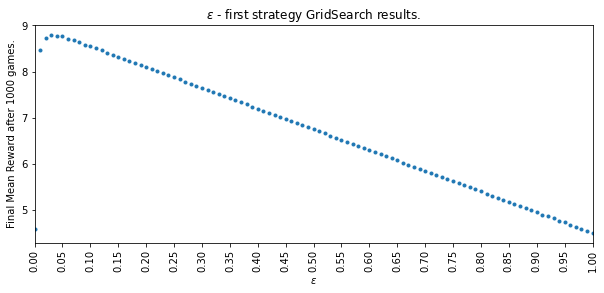
\includegraphics[scale=0.55]{e_fisrt.png}
	\caption{The performance of different $\varepsilon$-first strategies.}\label{fig::e_first}
\end{figure}

\subsubsection*{The best $\varepsilon$-greedy strategy}
Similarly as in previous method, we are exploring the possible values of $\varepsilon=0.00, 0.01, 0.02,\dots, 1.00.$ However the role of $\varepsilon$ slightly changes. In the following Figure \ref{fig::e_greedy} the final mean reward (after $1~000$ games) is presented. Based on the results, we declare $\varepsilon = 0.07$ the best option with the respect to the setting of the game and experiment.

\begin{figure}[h]
	\centering
	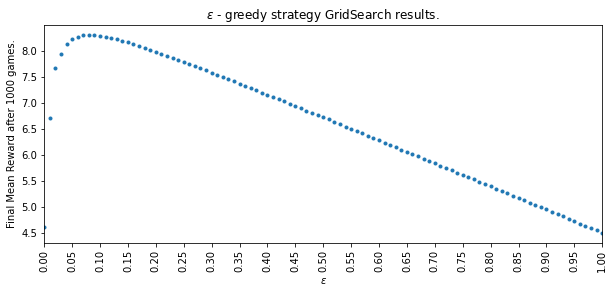
\includegraphics[scale=0.55]{e_greedy.png}
	\caption{The performance of different $\varepsilon$-greedy strategies.}\label{fig::e_greedy}
\end{figure}

\subsubsection*{The best $\varepsilon$-decay strategy}
More neck-to-neck situation can be observed in the $\varepsilon$-decay strategy. Based in the results visible in the Figure \ref{fig::e_decay} we declare $\beta = 0.12$ the best option with the respect to the setting of the game and experiment.

\begin{figure}[h]
	\centering
	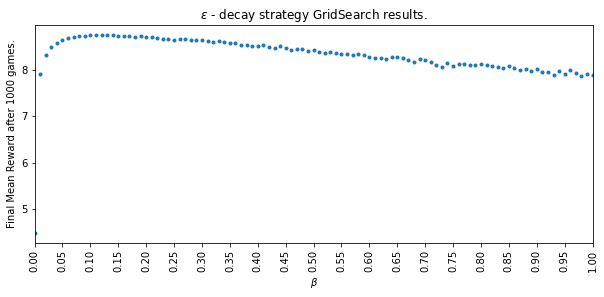
\includegraphics[scale=0.55]{e_decay.png}
	\caption{The performance of different $\varepsilon$-decay strategies.}\label{fig::e_decay}
\end{figure}

\newpage
\subsubsection*{The best SoftMax strategy}
In the SoftMax strategy the parameter called Temperature is being optimized. Firstly, Grid Search is used similarly as in previous cases. Based on this approach, the best value for temperature is $T=1.2$.
\begin{figure}[h]
	\centering
	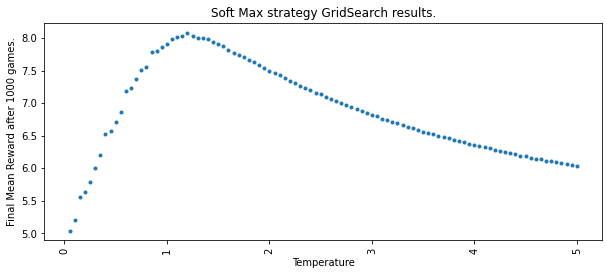
\includegraphics[scale=0.6]{SM.png}
	\caption{The performance of the temperature parameter setting for SoftMax strategy.}\label{fig::SM}
\end{figure}

Additionally, a different approach, the genetic algorithms, was tried. The genetic algorithms are commonly used to generate high-quality solutions to optimization and search problems by relying on biologically inspired operators such as mutation, crossover and selection. In the Figure \ref{fig::ga} (which was stolen from our lectures [7.]), is described the idea behind GA:

\begin{figure}[h]
	\centering
	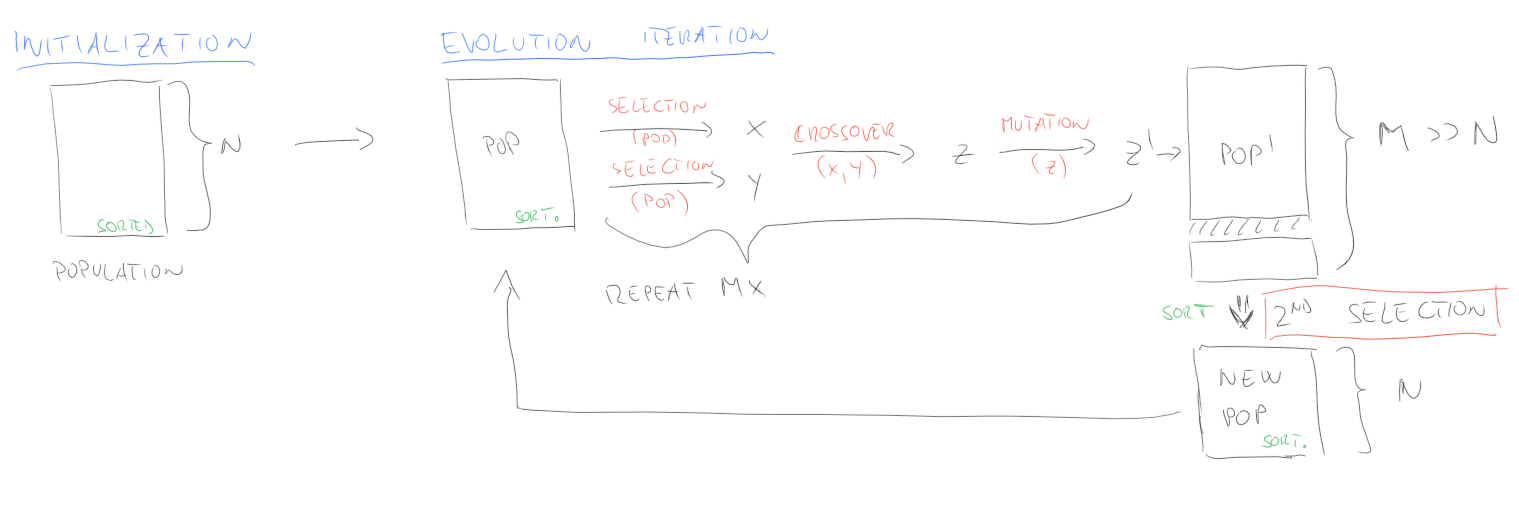
\includegraphics[scale=0.5]{go_overview.png}
	\caption{The genetic optimization.}\label{fig::ga}
\end{figure}

 The geneticalgorithm library offers an implementation of GA, the documentation can be found here: https://github.com/rmsolgi/geneticalgorithm. Following parameters are set:
 \begin{itemize}
 	\item objective function: (-1)*[the mean reward after 1000 rounds]
 	\item variable\_boundaries: [0.5, 1.5]
 	\item population\_size: 100
 	\item mutation\_probability: 0.1
 	\item elit\_ratio: 0.01
 	\item crossover\_probability: 0.5
 	\item parents\_portion: 0.3
 	\item crossover\_type': 'uniform'
 \end{itemize}

The results can be seen in the Figure \ref{fig::gaO}. Based on GA, best option is $T=1.21448554$. 

\begin{figure}[h]
	\centering
	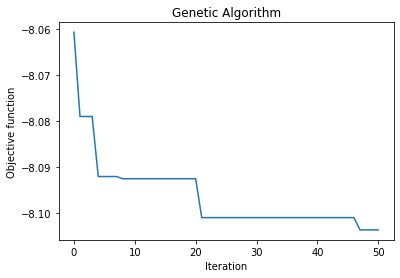
\includegraphics[scale=0.6]{ga1.png}
	\caption{The convergence of GA parameter search.}\label{fig::gaO}
\end{figure}

\subsection*{Summary}

For each strategy, the best possible setting of parameters was tested. In the last Figure \ref{fig::all} is the final comparison between the winning strategies. The best strategy (with respect to the setting of the experiment) is the $0.03$- first strategy with the final mean reward equal to $8.7923$.

\begin{figure}[h]
	\centering
	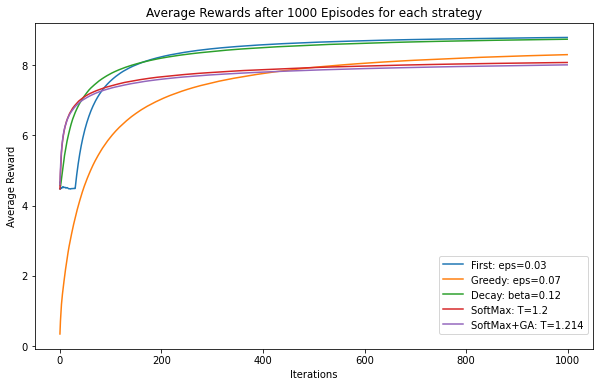
\includegraphics[scale=0.55]{summary.png}
	\caption{The final comparison of strategies.}\label{fig::all}
\end{figure}



	\clearpage
	\section*{References}
	\begin{enumerate}
		\item[1.] \textbf{Ritvik Kharkar}, A.A. [ritvikmath], Multi-Armed Bandit: Data Science Concepts (2020/09/23), YouTube, https://www.youtube.com/watch?v=e3L4VocZnnQ\&ab\_channel=ritvikmath
		\item[2.] \textbf{Robert C. Gray}, A.A. [Academic Gamer], Multi-Armed Bandits: A Cartoon Introduction - DCBA \#1 (2020/08/08), YouTube, \\https://www.youtube.com/watch?v=bkw6hWvh\_3k\&ab\_channel=AcademicGamer
		\item[3.] \textbf{Aleksandrs Slivkins}, Introduction to Multi-Armed Bandits, Microsoft Research NYC, Version September 2019, 2017-2019
		\item[4.] \textbf{João Gama, Rui Camacho, Pavel B. Brazdil, Alípio Mário Jorge, Luís Torgo}, Machine Learning: ECML 2005, 16th European Conference on Machine Learning, Proceedings, Porto, Portugal, October 3-7, 2005, 0302-9743
		\item[5.] HEUR Lectures, 2022
		\item[6.] https://en.wikipedia.org/wiki/Hyperparameter\_optimization
	\end{enumerate}
	
\end{document}